\documentclass[11pt]{article}
\usepackage{layout}

\usepackage[top=3cm, bottom=3cm, left=4cm, right=2cm]{geometry}

\usepackage{amsmath}
\usepackage{amssymb}
\usepackage{mathrsfs}
\usepackage{amsthm}
\usepackage[utf8]{inputenc}
%\usepackage[latin1]{inputenc} 
\usepackage[T1]{fontenc}  
\usepackage[french]{babel}
\usepackage{titlesec}
\usepackage[pdftex]{graphicx}
\usepackage{graphics}
\usepackage{float}
\usepackage{bbm}


\newtheorem{scenario}{Scénario}
\newtheorem{exemple}{Exemple}

\begin{document}
\renewcommand{\tablename}{Tableau}
\renewcommand{\figurename}{Illustration}

	\begin{titlepage}
		\centering % Centre everything on the title page
		
		\scshape % Use small caps for all text on the title page
		
		\vspace*{7\baselineskip} % White space at the top of the page
		
		%------------------------------------------------
		%	Title
		%------------------------------------------------
		
		\rule{\textwidth}{1.6pt}\vspace*{-\baselineskip}\vspace*{2pt} % Thick horizontal rule
		\rule{\textwidth}{0.4pt} % Thin horizontal rule
		
		\vspace{0.75\baselineskip} % Whitespace above the title
		{\LARGE Estimation des paramètres par la méthode composite \\} % Title
		\vspace{0.75\baselineskip} % Whitespace below the title
		
		\rule{\textwidth}{0.4pt}\vspace*{-\baselineskip}\vspace{3.2pt} % Thin horizontal rule
		\rule{\textwidth}{1.6pt} % Thick horizontal rule
		
		\vspace{3\baselineskip} % Whitespace after the title block
		
		%------------------------------------------------
		%	Subtitle
		%------------------------------------------------
		{\scshape\Large Sous la supervision de \\ Hélène Cossette\\Étienne Marceau\\ } % Editor list
		
		\vspace*{3\baselineskip}
		
		  % Subtitle or further description
		
		\vspace*{3\baselineskip} % Whitespace under the subtitle
		
		%------------------------------------------------
		%	Editor(s)
		%------------------------------------------------
		
		Préparé par
		
		\vspace{0.5\baselineskip} % Whitespace before the editors
		
		{\scshape\Large Alexandre Lepage, \\
			Diamilatou N'diaye, \\} % Editor list
		
		\vspace*{5\baselineskip}
		
		le 03 Juillet 2019
		
		\vspace{0.5\baselineskip} % Whitespace below the editor list
		
		\vfill % Whitespace between editor names and publisher logo
		
		%------------------------------------------------
		%	Publisher
		%------------------------------------------------
		
		
\includegraphics[height=1.2cm]{graph/UL_P.pdf}\\
		
		Faculté des sciences et de génie\\
		École d'actuariat\\
		Université Laval\\     
	\end{titlepage}
	
	%\setcounter{secnumdepth}{0} % sections are level 1
	%\setcounter{section}{1}
	
	\pagenumbering{Roman} % Pagination en chiffres romains
	\setcounter{page}{0}
	
	\newpage
	\strut % Page blanche
	\newpage
	
	\tableofcontents
	\newpage
	\renewcommand{\listfigurename}{Liste des illustrations}
	\listoffigures
	\newpage
	\listoftables
	\newpage
	
	\pagenumbering{arabic} % Pagination en chiffres normaux
	\setcounter{page}{1}

\section{Estimation par la Méthode Composite} \label{sect_description_scenario}

	Le but de ce rapport est de présenter les résultats d'estimation des paramètres d'un modèle collectif du risque tel que décrit dans \cite{Itre5} avec la méthode composite présentée dans \cite{LikelyhoodEstimation}. Dans les exemples suivants, $N \sim Binom(5,q), \ q=0.2$ et $X \sim Exp(\beta) , \ \beta=1/100$. La copule hiérarchique étudiée est construite à partir d'une v.a. mère qui suit une loi géométrique de paramètre $\alpha_{0}=0.6$ et d'une v.a. enfant qui suit une loi géométrique de paramètre $\alpha_{1}=0.4$. Les estimations sont réalisées sur un échantillon simulé de $10\,000$ observations.

\section{Première Approche : Méthode \textit{IFM}}
	
	La première approche consiste à estimer séparément tous les paramètres. Dans un premier temps, les paramètres $q$ et $\beta$ sont estimés pas les estimateurs du maximum de vraisemblance de leur loi respectives. 
	\[ \hat{q} = \frac{\sum^{n_{obs}}_{i=0} n_{i}}{5\times n_{obs}}, \]
	\[ \hat{\beta} = \frac{\sum^{n_{obs}}_{i=0} n_i}{\sum^{n_{obs}}_{i=0} \sum_{j=1}^{n_i} x_{i,j}} \]
	où $n_{obs}$ représente le nombre d'observations ($i$) présents dans l'échantillon, $n_i$ représente la $i^e$ réalisation de $N$ et $x_{i,j}$ correspond au $j^e$ sinistre de la $i^e$ observation de la v.a. $X$.\\
	
	Ensuite l'estimateur de $\alpha_{0}$ est obtenu en maximisant la fonction de vraisemblance \eqref{eq_vrais_alpha0_1}.
	\begin{equation}\label{eq_vrais_alpha0_1}
		L(\alpha_{0} \vert \hat{q},\hat{\beta}) = \prod^{n_{NX}}_{i=1} \left(\frac{\partial}{\partial x} C(F_{N}(n_{i} \vert \hat{q}),F_{X}(x_{i} \vert \hat{\beta})) - \frac{\partial}{\partial x} C(F_{N}(n_{i}-1 \vert \hat{q}),F_{X}(x_{i} \vert \hat{\beta}))\right)
	\end{equation}

	où $n_{NX}$ représente le nombre de couples $(N_{i},X_{i,j})$ présents dans l'échantillon.\\
	
	De plus, avec le modèle collectif du risque définit par $S= \sum_{j=1}^{\infty} X_{j} \times \mathbbm{1}\{j \leq N\}$, la copule reliant la v.a. $N$ avec n'importe lequel des $X_{j}$ s'exprime comme
	
	\begin{equation}\label{eq_copule_NX}
		C(u_{0},u_{1}) = \mathscr{L}_{M}(\mathscr{L}_{M}^{-1}(u_{0}) + \mathscr{L}_{M}^{-1}(u_{1}) ).
	\end{equation}

	À noter que la copule décrite en \eqref{eq_copule_NX} est archimédienne.\\
	
	Et enfin, de la même manière que pour $\alpha_{0}$, l'estimateur de $\alpha_{1}$ est obtenu en maximisant la fonction de vraisemblance \eqref{eq_vrais_alpha1_1}.
	
	\begin{equation}\label{eq_vrais_alpha1_1}
		L(\alpha_{1} \vert \hat{\beta},\hat{\alpha_{0}}) = \prod^{n_{XX}}_{i=1} \frac{\partial^2}{\partial x_{1}\partial x_{2}} C(F_{X}(x_{1i} \vert \hat{\beta}),F_{X}(x_{2i}\vert \hat{\beta}) \vert \hat{\alpha_{0}}),
	\end{equation}
	où $n_{XX}$ représente le nombre de couples $\{(X_{i,k},X_{i,j}): k \neq j\}$ présents dans l'échantillon.
	
	\[ C(u_{1},u_{2} \vert \hat{\alpha_{0}}) = \mathscr{L}_{\Theta\vert \hat{\alpha_{0}}}(\mathscr{L}_{\Theta \vert \hat{\alpha_{0}}}^{-1}(u_{1} ) + \mathscr{L}_{\Theta\vert \hat{\alpha_{0}}}^{-1}(u_{2} ) ), \]
	 avec    \[ \mathscr{L}_{\Theta\vert \hat{\alpha_{0}}}(t) = \mathscr{L}_{M\vert \hat{\alpha_{0}}}(-\ln(\mathscr{L}_{B}(t))) \]
	 
	 et $$ \mathscr{L}^{-1}_{\Theta \vert \hat{\alpha_{0}}}(u) = \mathscr{L}_B^{-1}\left(exp(-\mathscr{L}^{-1}_{M \vert \hat{\alpha_{0}}}(u)) \right). $$
	
	Le tableau \ref{resultats_app1} présente les valeurs des estimateurs.
	
	\begin{table}[H]
		\centering
		\begin{tabular}{lrrrr}
			  \hline
			 & $q$ & $\beta$ & $\alpha_{0}$ & $\alpha_{1}$ \\ 
			  \hline
			  Valeur & 0.2000 & 0.0100 & 0.6000 & 0.4000 \\ 
			  Estimateur & 0.1996 & 0.0087 & 0.3603 & 0.8545 \\ 
			  Temps & 0.0000 & 0.0000 & 1.3900 & 0.7900 \\ 
			   \hline
		\end{tabular}
 		\caption{Valeurs estimées de $q$, $\beta$, $\alpha_{0}$, $\alpha_{1}$ ainsi que le temps de calcul par la première approche.}
	 	\label{resultats_app1}
	\end{table}

	On voit en regardant le tableau \ref{resultats_app1} que les résultats de l'estimation sont loins des vrais paramètres.\\


\subsection{Comportement Asympotique}

	La méthode précédente est répétée 100 fois afin d'observer le comportement asymptotique des estimateurs.
	Pour $\alpha_{0}$,  on obtient une moyenne de 0.3556106 et un intervalle de confiance de niveau $ \alpha = 95\% $ de $[0.3117377,0.3994836]$.
	
	\begin{figure}[H]
		\centering
		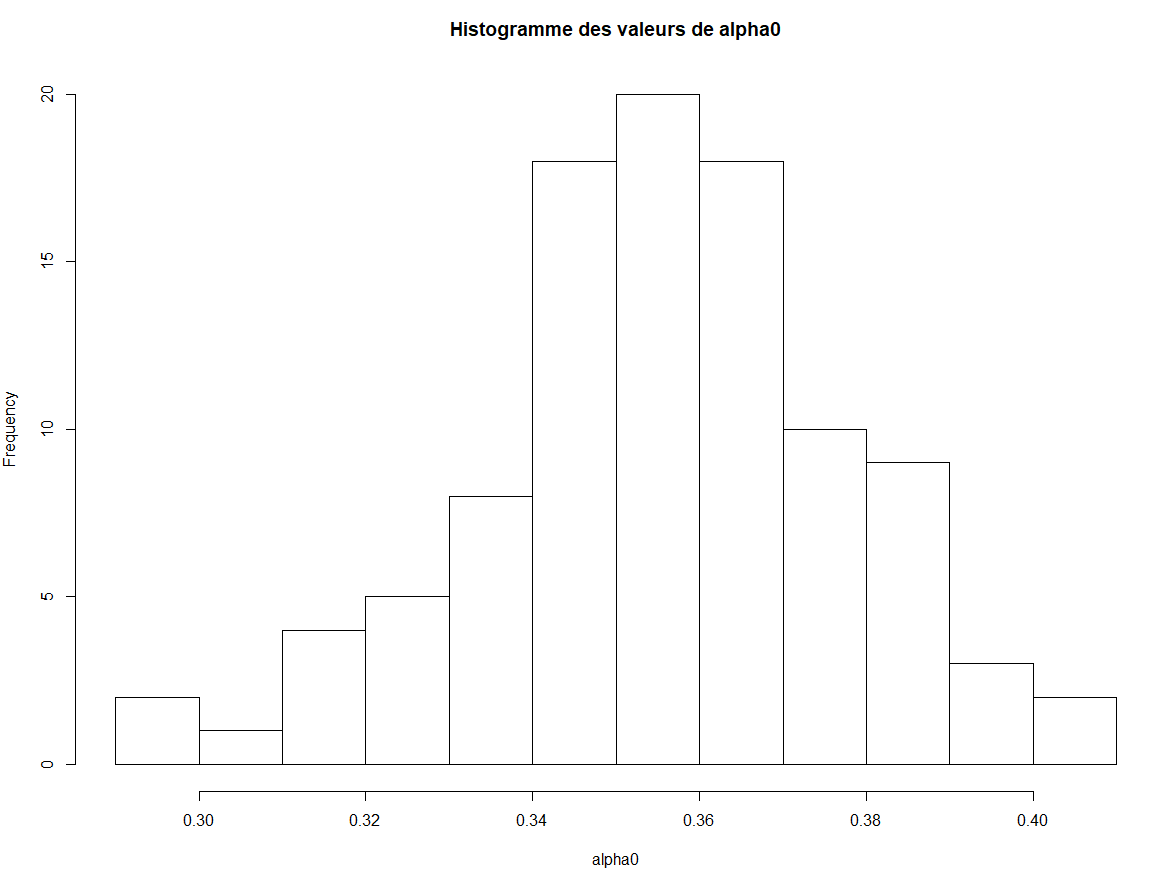
\includegraphics[height=6cm]{graph/alpha0.png}
		\caption[Paramètre $\alpha_{0}$]{Histogramme des valeurs prises par $\alpha_{0}$ sur 100 répétitions} 
		\label{alpha0}
	\end{figure}
		
	Pour $\alpha_{1}$ on obtient une moyenne de  0.8201792 et un intervalle de confiance de niveau $\alpha = 95\% $ de $[0.7704843,0.8698740]$.

	\begin{figure}[H]
		\centering
		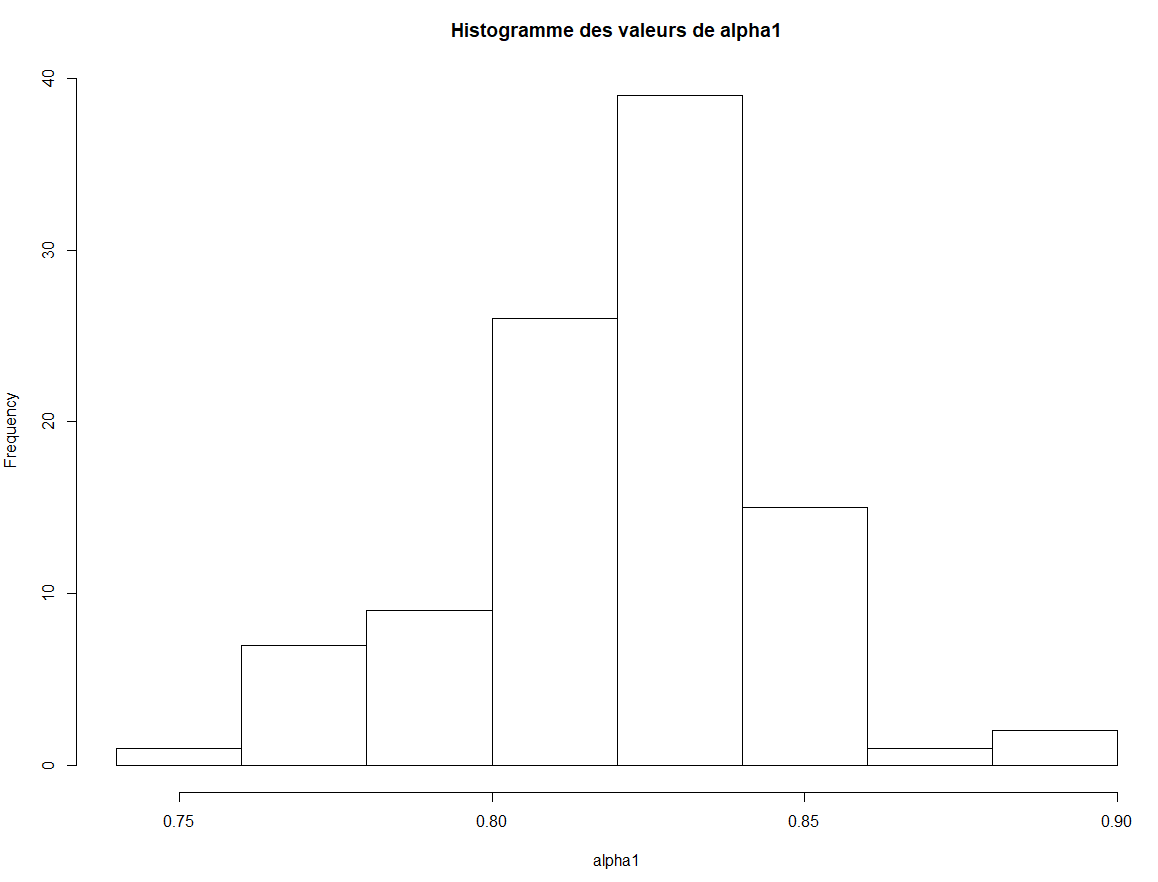
\includegraphics[height=6cm]{graph/alpha1.png}
		\caption[Paramètre $\alpha_{1}$]{Histogramme des valeurs prises par $\alpha_{1}$ sur 100 répétitions} 
		\label{alpha1}
	\end{figure}
		

\subsubsection{Comportement asymptotique des estimateurs pour une copule archimédienne hiérarchique Logarithmique-Gamma de paramètres $(\alpha_{0}=6,\alpha_{1}=4)$}

	L'estimateur de $\alpha_{0}$ produit une moyenne de 3.232702 et un intervalle de confiance de niveau $ \alpha = 95\% $ de $[3.114684,3.350721]$.
	
	\begin{figure}[H]
		\centering
		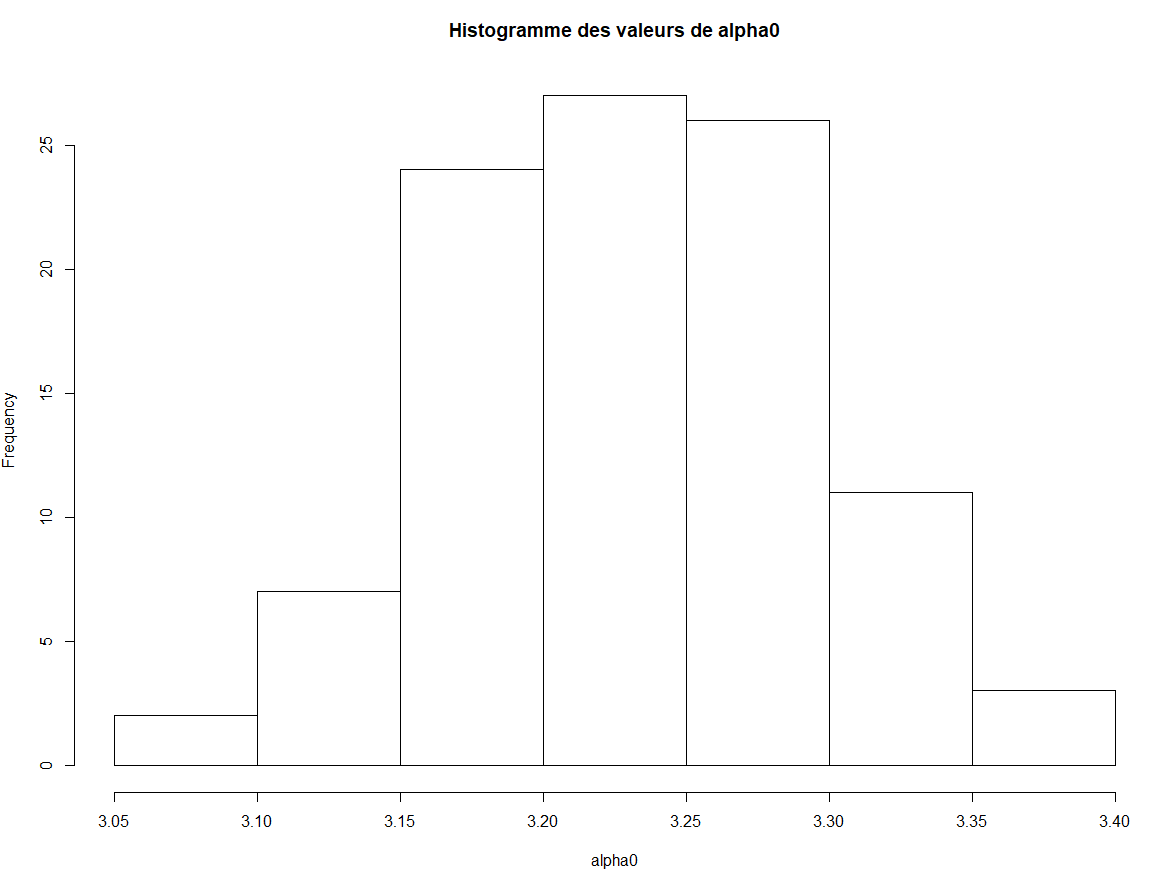
\includegraphics[height=6cm]{graph/alpha0lg.png}
		\caption[Paramètre $\alpha_{0}$]{Histogramme des valeurs prises par $\alpha_{0}$ sur 100 répétitions} 
		\label{alpha0lg}
	\end{figure}
		
	L'estimateur de $\alpha_{1}$ produit  une moyenne de  6.646969 et un intervalle de confiance de niveau $\alpha = 95\% $ de $[6.094799,7.199139]$.

	\begin{figure}[H]
		\centering
		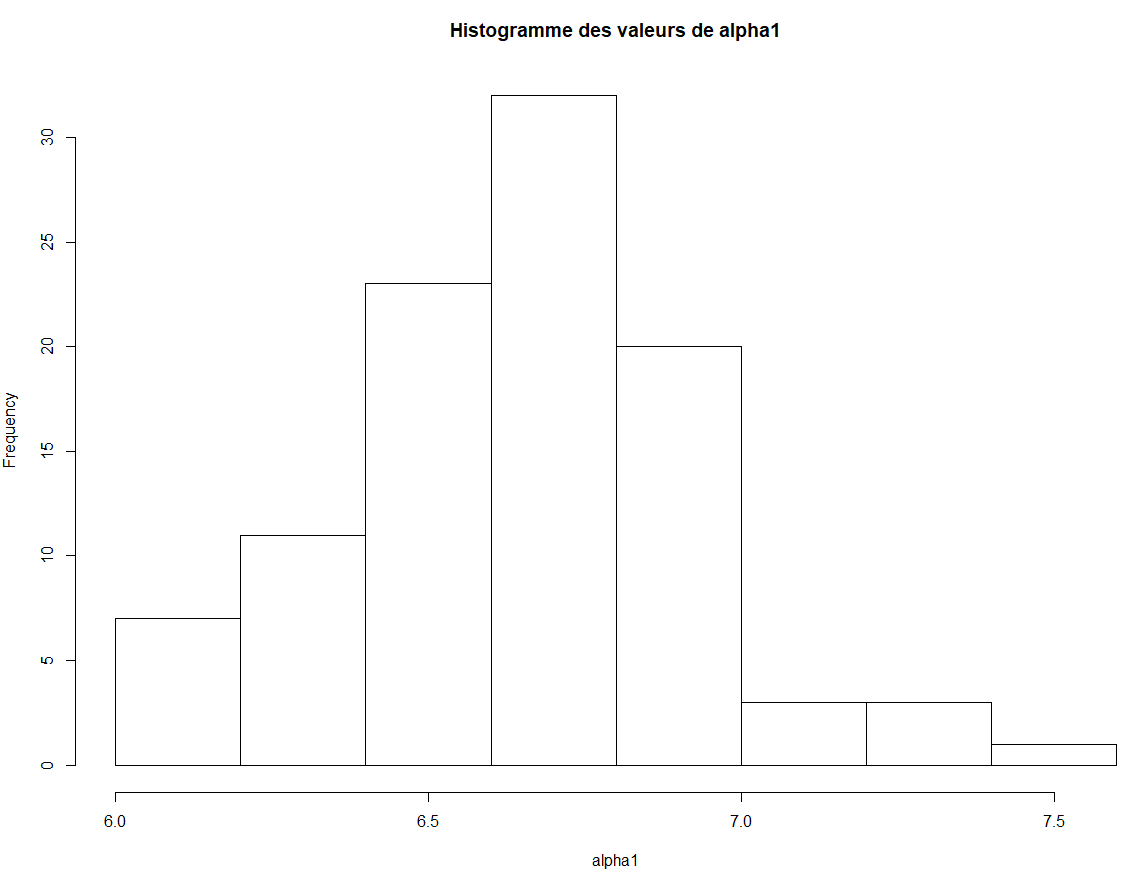
\includegraphics[height=6cm]{graph/alpha1lg.png}
		\caption[Paramètre $\alpha_{1}$]{Histogramme des valeurs prises par $\alpha_{1}$ sur 100 répétitions} 
		\label{alpha1lg}
	\end{figure}
		
	Les estimations sont donc assez loin des vrais paramètres. 

\section{Seconde Approche: Méthode composite}\label{sect_seconde_approche}

	La seconde approche consiste à estimer $q$, $\beta$ et $\alpha_{0}$ en même temps puis $\alpha_{1}$ par la suite. 
	La fonction de vraisemblance à maximiser  est :
	
	
\[ L(\alpha_{0},q,\beta) =\prod^{n_{NX}}_{i=1} \left(\frac{\partial}{\partial x} C(F_{N}(n_{i}),F_{X}(x_{i})) - \frac{\partial}{\partial x} C(F_{N}(n_{i}-1),F_{X}(x_{i}))\right) \]
	où $n_{NX}$ représente le nombre de couples $(N_{i},X_{i,j})$ présents dans l'échantillon.
	\[ C(u_{0},u_{1}) = \mathscr{L}_{M}(\mathscr{L}_{M}^{-1}(u_{0}) + \mathscr{L}_{M}^{-1}(u_{1}) ). \]
	
	Pour ce qui est de $\alpha_{1}$, la même estimation que la section précédente est réalisée.
	
	\begin{equation} \label{eq_vrais_alpha1_2}
	L(\alpha_{1}, \beta, \alpha_{0}) = \prod^{n_{XX}}_{i=1} \frac{\partial^{2}}{\partial x_{1}\partial x_{2}} C(F_{X}(x_{1i}),F_{X}(x_{2i})),
	\end{equation}
	
	où $$C(u_{1},u_{2}) = \mathscr{L}_{\Theta}(\mathscr{L}_{\Theta}^{-1}(u_{1}) + \mathscr{L}_{\Theta}^{-1}(u_{2}) ),$$
	avec    \[ \mathscr{L}_{\Theta}(t) = \mathscr{L}_{M}(-\ln(\mathscr{L}_{B}(t))) \]
	et $n_{XX}$ représente le nombre de couples $(X_{i,k},X_{i,j})$ présents dans l'échantillon. Le tableau \ref{resultats_app1} présente les valeurs des estimateurs;

	\begin{table}[H]
		\centering
		\begin{tabular}{rrrrr}
		  \hline
		 	& $q$ & $\beta$ & $\alpha_{0}$ & $\alpha_{1}$ \\  
		  \hline
			Valeur & 0.2000 & 0.0100 & 0.6000 & 0.4000 \\ 
			Estimateur & 0.3589 & 0.0087 & 0.4972 & 0.8000 \\ 
			Temps & 45.6000 & 45.6000 & 45.6000 & 1.4100 \\ 
		   \hline
		\end{tabular}
	 		\caption{Valeurs estimées de $q$, $\beta$, $\alpha_{0}$, $\alpha_{1}$ ainsi que le temps de calcul par la deuxième approche. Le temps de calcul de $q$, $\beta$ et $\alpha_{0}$ est leur temps de calcul commun étant donné qu'ils sont estimés ensembles.}
	 	\label{resultats_app2}
	\end{table}

	Dans le tableau \ref{resultats_app2}, on voit que le niveau de précision est légèrement meilleur que pour la première approche lorsque l'on regarde $\alpha_{0}$ et $\alpha_{1}$, bien que ce ne soit toujours pas satisfaisant. Tandis que pour $\hat{q}$, les résultats se détériorent.

\subsection{Comportement Asympotique}

	L'estimation est ensuite répétée 100 fois afin d'observer le comportement asymptotique des estimateurs.
	L'estimateur de $\alpha_{0}$ produit une moyenne de 0.4856781 et un intervalle de confiance de niveau $\alpha = 95\%$ de $[0.3888275,0.5825286]$.
	
	\begin{figure}[H]
		\centering
		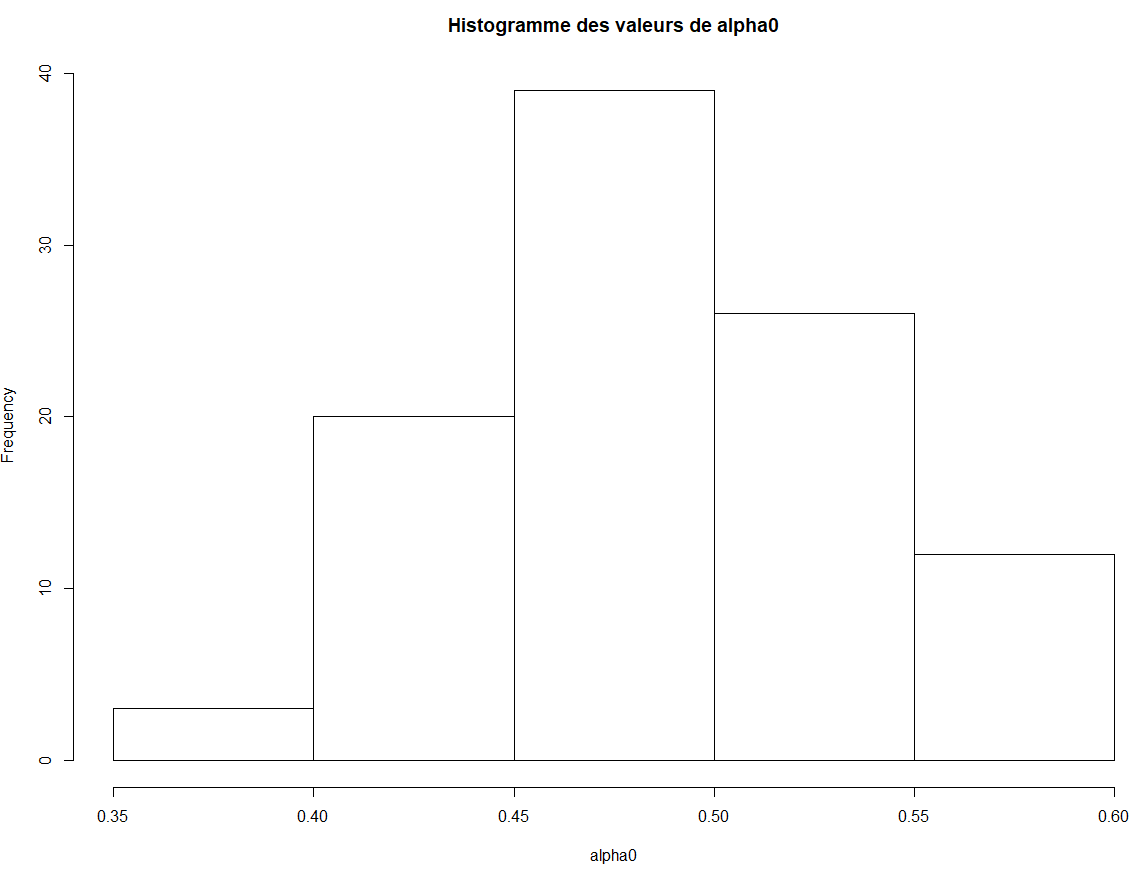
\includegraphics[height=6cm]{graph/alpha02.png}
		\caption[Paramètre $\alpha_{0}$]{Histogramme des valeurs prises par $\alpha_{0}$ sur 100 répétitions} 
		\label{alpha02}
	\end{figure}
		
	L'estimateur de $\alpha_{1}$ produit une moyenne de  0.7690707 et un intervalle de confiance de niveau $\alpha = 95\%$ de $[0.7103108,0.8278306]$.

	\begin{figure}[H]
		\centering
		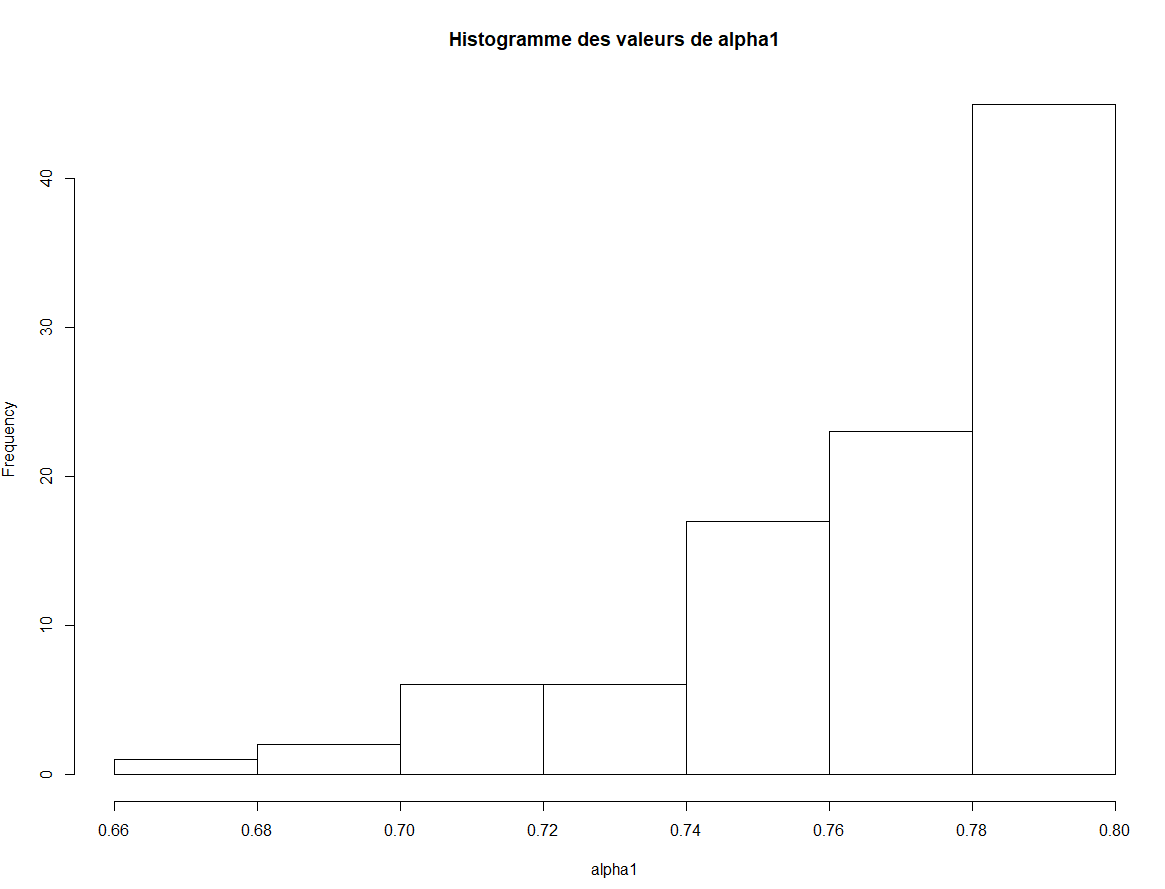
\includegraphics[height=6cm]{graph/alpha12.png}
		\caption[Paramètre $\alpha_{1}$]{Histogramme des valeurs prises par $\alpha_{1}$ sur 100 répétitions} 
		\label{alpha12}
	\end{figure}


\section{Impact de la paramétrisation de la loi de fréquence}
	
	Dans \cite{nikoloulopoulos2009modeling}, il est fait mention que la distribution marginale des variables aléatoires discrètes ont un impact sur le calcul des taux de Kendall à cause de l'existence de valeurs identiques. Dans le scénario présenté dans la section \ref{sect_description_scenario}, cette problématique se manifeste comme il est possible de le voir dans l'illustration \ref{graph_kendall_va_mixtes}. En effet, on y voit que plus le paramètre de probabilité $q$ est petit, plus le tau de Kendall est sous-estimé dans le calcul empirique. Cela est assimilable au grand nombre d'observations de $N$ qui sont égales à zéro. Ce problème se manifeste non seulement dans cette mesure de dépendance, mais aussi dans l'estimation des paramètres de la copule.
	
	 \begin{figure}[H]
	 	\centering
	 	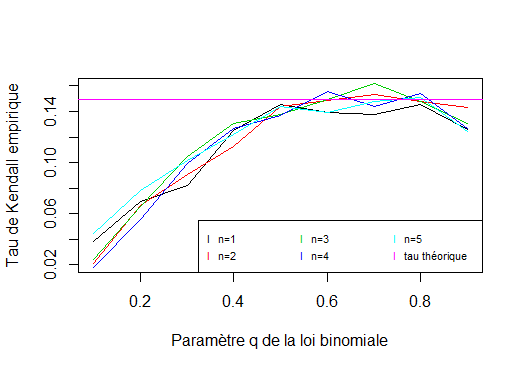
\includegraphics[height=7cm]{graph/Tau_kendall_empirique.png}
	 	\caption[Effet de la paramétrisation de la loi de fréquence sur le calcul du tau de Kendall empirique.]{Effet de la paramétrisation de la loi de fréquence sur le calcul du tau de Kendall empirique: les graphiques sont réalisés avec $30 \times 5 \times 10$ simulations de 100 observations d'une copule AMH avec une première variable aléatoire qui suit une loi binomiale($n,q$) et une seconde qui suit une loi exponentielle de moyenne 100, où $n = 1, \dots, 5$ et q = $\frac{1}{10}, \frac{2}{10}, \dots, \frac{9}{10}$. Le tau théorique, présenté sous forme de ligne droite rose, est calculé avec une loi binomiale($n=5, q=3/5$). Ce dernier varie très peu en fonction de $q$, mais beaucoup en fonction de $n$.} 
	 	\label{graph_kendall_va_mixtes}
	 \end{figure}
 	
 	Posons maintenant deux scénarios pour illustrer cette problématique sur l'estimation des paramètres dans le contexte d'un modèle collectif du risque décrit dans \cite{Itre5}.
 	
 	\begin{scenario}
 		\textbf{$N \sim Binomiale(5, 0.2)$}
 	\end{scenario}
 		Pour le premier scénario, reprenons la paramétrisation décrite dans la section \ref{sect_description_scenario}. On obtient donc le tableau de résultats présenté dans le tableau \ref{tbl_resultats_scenario_1}\footnote{À noter que les résultats diffèrent légèrement de ceux présentés dans les tableaux \ref{resultats_app1} et \ref{resultats_app2} du fait que les simulations n'ont pas le même encrage (\textit{seed}) et que le code utilisé est différent.}.
 		
 		\begin{table}[H]
 			\centering
 			\begin{tabular}{lcccc}
 				\hline
 				& $q$ & $\beta$ & $\alpha_0$ & $\alpha_1$ \\ 
 				\hline
 				Vrais paramètres & 0.2000 & 0.0100 & 0.6000 & 0.4000  \\ 
 				Méthode \textit{IFM} & 0.1980 & 0.0090 & 0.4241 & 0.8407  \\ 
 				Méthode composite & 0.2972 & 0.0090 & 0.5487 & 0.7911 \\ 
 				Méthode des moments & 0.1980 & 0.0087 & 0.2752 & 0.4339 \\ 
 				\hline
 			\end{tabular}
 			\caption[Résultats du premier scénario.]{Résultats du premier scénario: La méthode dite \textit{IFM} consiste à trouver les paramètres des distributions marginales, puis à estimer $\hat{\alpha}_{0}$ sachant ces paramètres. De la même façon, on trouve $\hat{\alpha}_{1}$ en fixant $\beta$ et $\alpha_{0}$ comme connus. La méthode dite \textit{composite}, quant à elle, consiste à trouver tous les paramètres simultanément en utilisant la méthode décrite dans la section \ref{sect_seconde_approche}. Finalement, la méthode des moments, dans les cas de $\hat{\alpha}_{0}$ et $\hat{\alpha}_{1}$, consiste à inverser le tau de Kendall empirique.}
 			\label{tbl_resultats_scenario_1}
 		\end{table}
 	
 	Dans le tableau \ref{tbl_resultats_scenario_1}, on voit que ni la méthode des moments ni la méthode \textit{IFM} ne donne de bons résultats pour estimer $\alpha_0$. De ce fait, on ne peut obtenir de bons paramètres de départ pour l'optimisation numérique de la méthode composite. Malgré tout, cette dernière donne un résultat relativement prêt du vrai paramètre. Cependant, lorsque l'on regarde l'estimation de $q$ sous cette méthode, celle-ci s'éloigne du vrai paramètre.\\
 	
 	Dans ce contexte (où on a une loi de fréquence qui a une masse à zéro élevée), l'approche recommandée est de trouver le paramètre de la distribution de la loi de fréquence avec sa fonction de vraisemblance marginale (en ignorant les autres paramètres), puis d'utiliser la méthode composite pour estimer les autres paramètres.
 	
 	 \begin{scenario}
 		\textbf{$N \sim Binomiale(5, 0.6)$}
 	\end{scenario}
 		Pour le second scénario, on reprend la même paramétrisation que pour le premier, mais on remplace $q=0.2$ pour $q=0.6$.
 		On obtient alors les résultats présentés dans le tableau \ref{tbl_resultats_scenario_2}.
 	
 	 \begin{table}[H]
 		\centering
 		\begin{tabular}{lcccc}
 			\hline
 			& $q$ & $\beta$ & $\alpha_0$ & $\alpha_1$ \\ 
 			\hline
 			Vrais paramètres & 0.6000 & 0.0100 & 0.6000 & 0.4000 \\ 
 			Méthode \textit{IFM} & 0.5984 & 0.0099 & 0.5980 & 0.6026 \\ 
 			Méthode composite & 0.6037 & 0.0100 & 0.5825 & 0.6117 \\ 
 			Méthode des moments & 0.5984 & 0.0094 & 0.5789 & 0.4427 \\
 			\hline
 		\end{tabular}
 		\caption[Résultats du deuxième scénario.]{Résultats du deuxième scénario: La méthode dite \textit{IFM} consiste à trouver les paramètres des distributions marginales, puis à estimer $\hat{\alpha}_{0}$ sachant ces paramètres. De la même façon, on trouve $\hat{\alpha}_{1}$ en fixant $\beta$ et $\alpha_{0}$ comme connus. La méthode dite \textit{composite}, quant à elle, consiste à trouver tous les paramètres simultanément en utilisant la méthode décrite dans la section \ref{sect_seconde_approche}. Finalement, la méthode des moments, dans les cas de $\hat{\alpha}_{0}$ et $\hat{\alpha}_{1}$, consiste à inverser le tau de Kendall empirique.}
 		\label{tbl_resultats_scenario_2}
 	\end{table}
 	
 	Ce que l'on remarque dans le tableau \ref{tbl_resultats_scenario_2}, c'est que toutes les estimations sont plus près des vrais paramètres, même pour $\alpha_1$. 	
 	Cela est explicable du fait qu'il y a plus d'observations pour $X$; ce qui permet un meilleur ajustement pour $\hat{\beta}$. Cela a des répercussions sur le calcul du maximum de vraisemblance des autres paramètres. Par la suite, on a des meilleures valeurs de départ pour la méthode composite puisque le tau de Kendall est plus crédible. Finalement, l'estimation de $\alpha_1$ s'est amélioré étant donnée que les autres paramètres selon lesquels sa vraisemblance dépend sont mieux ajustés. Dans ce contexte, la méthode composite est l'approche la plus adéquate pour estimer les paramètres du modèle.
 	Cependant, on voit que la méthode de calcul de la vraisemblance proposé en \eqref{eq_vrais_alpha1_1} et en \eqref{eq_vrais_alpha1_2} ne donne pas de bons résultats. Il faudra donc trouver une méthode alternative pour estimer adéquatement $\alpha_1$.
 	
 	\section{Impact du choix de la copule et des paramètres de dépendance}
 		Dans le cas d'un modèle où la loi mère est géométrique, comme le niveau de dépendance n'est pas très élevé, même avec un paramètre $\alpha_0$ avoisinant $1$, on n'observe pas de biais dans l'estimation de $\beta$. Cependant, lorsque la loi mère de la copule archimédienne hiérarchique est logarithmique, la dépendance est plus forte. Il s'ensuit que les valeurs que peut prendre la v.a. $X_{i,j}$ seront davantage influencées par les valeurs que prendra la v.a. $N_i$, i=1,\dots, $n_{obs}$, comme l'illustre l'exemple \ref{exemple_1}.
 		
 		\begin{exemple}\label{exemple_1}
 			On a une copule archimédienne hiérarchique logarithmique-logarithmique avec $\alpha_0 = 10$ et $\alpha_1 = 10$. Les variables aléatoires sous-jacentes sont $N \sim binomiale(n=5, q=3/5)$ et $X \sim exponentielle(1/100)$. On simule $10\,000$ réalisations d'un tel modèle. Le tableau \ref{tbl_head_exemple1} présente les six premiers résultats de l'exemple \ref{exemple_1}.
 			
 			\begin{table}[H]
 				\centering
 				\begin{tabular}{rrrrrrr}
 					\hline
 					i & N & X1 & X2 & X3 & X4 & X5 \\ 
 					\hline
 					1 & 2 & 8.14 & 9.45 &  &  &  \\ 
 					2 & 5 & 314.10 & 627.06 & 205.52 & 487.95 & 257.58 \\ 
 					3 & 4 & 192.08 & 189.38 & 251.15 & 173.13 &  \\ 
 					4 & 2 & 69.24 & 82.65 &  &  &  \\ 
 					5 & 3 & 100.02 & 85.79 & 204.63 &  &  \\ 
 					6 & 4 & 166.59 & 159.45 & 272.40 & 217.62 &  \\ 
 					\hline
 				\end{tabular}
 			\caption{Six premières réalisations de l'exemple \ref{exemple_1}.}
 			\label{tbl_head_exemple1}
 			\end{table}
 		
 			Dans le tableau \ref{tbl_head_exemple1}, on voit que, pour de grands $N_i$, les valeurs de $X_{i,j}$ sont également élevées. Conséquemment, on se retrouve donc avec un nombre plus élevé de grands $X$ comme l'illustre le tableau \ref{tbl_sommaire_exemple_1}. De cette façon, si on calcule le paramètre de la loi exponentielle avec la méthode du maximum de vraisemblance, on a $\hat{\beta} = 1 / \bar{x} = 1 / 125.0237 \neq 1/100.$
 			
 			\begin{table}[H]
 				\centering
 				\begin{tabular}{rrrrrrrr}
 					\hline
 					& Min. & 1st Qu. & Median & Mean & 3rd Qu. & Max. & NA's \\ 
 					\hline
 					N & 0.00 & 2.00 & 3.00 & 2.99 & 4.00 & 5.00 & 0.00 \\ 
 					X1 & 0.01 & 29.25 & 69.02 & 100.62 & 138.48 & 1108.40 & 106.00 \\ 
 					X2 & 0.00 & 37.07 & 78.76 & 108.29 & 147.52 & 1011.26 & 880.00 \\ 
 					X3 & 0.12 & 63.14 & 105.86 & 134.07 & 177.06 & 1056.53 & 3196.00 \\ 
 					X4 & 13.14 & 118.05 & 170.15 & 194.77 & 246.33 & 832.55 & 6686.00 \\ 
 					\hline
 				\end{tabular}
 			\caption{Sommaire des données simulées pour l'exemple \ref{exemple_1}.}
 			\label{tbl_sommaire_exemple_1}
 			\end{table}
 		
 		\end{exemple}
 	
 		Une méthode pour remédier à la situation présentée dans l'exemple \ref{exemple_1} consiste à prendre un $X_{i,j}$ au hasard pour chaque observation ($i$), puis de répéter cette expérience plusieurs fois (30 à 100 fois) afin de créer un vecteur de montants de sinistres où aucun quantile ne serait plus représenté qu'un autre. Finalement, on trouve la moyenne de ce nouveau vecteur pour obtenir un paramètre $\hat{\beta}$ plus représentatif des données. \\
 		
 		Voyons maintenant avec deux autres scénarios comment cela se traduit dans l'estimation de tous les paramètres d'un modèle collectif du risque.
 		
 		\begin{scenario}\label{scenario_tous_les_Xij}
 			On prend tous les $X_{i,j}$ pour calculer l'estimateur de $\beta$.
 		\end{scenario}
 			Posons un modèle collectif du risque où la copule archimédienne hiérarchique est logarithmique-logarithmique avec $\alpha_0 = 8$ et $\alpha_1=6$. Pour le scénario \ref{scenario_tous_les_Xij}, on prend l'approche classique où $\hat{\beta} = 1 / \bar{x}$ et que $\bar{x} = \sum_{i=1}^{n_{obs}} \sum_{j=1}^{N_i} x_{i,j}$. On prend alors en compte tous les $X_{i,j}$. Avec $1\,000$ observations simulées, on obtient les résultats présentés dans le tableau \ref{tbl_resultats_scenario_3}
 		
 			\begin{table}[H]
 				\centering
 				\begin{tabular}{lcccc}
 					\hline
 					& $q$ & $\beta$ & $\alpha_0$ & $\alpha_1$ \\ 
 					\hline
 					Vrais paramètres & 0.6000 & 0.0100 & 8.0000 & 6.0000 \\ 
 					Méthode \textit{IFM} & 0.6128 & 0.0078 & 7.3331 & 7.9825 \\ 
 					Méthode composite & 0.6132 & 0.0095 & 8.2209 & 7.2317 \\ 
 					Méthode des moments & 0.6128 & 0.0078 & 7.8535 & 4.2966 \\ 
 					\hline
 				\end{tabular}
 			\caption[Résultats du scénario \ref{scenario_tous_les_Xij}]{Résultats du scénario \ref{scenario_tous_les_Xij}: La méthode dite \textit{IFM} consiste à trouver les paramètres des distributions marginales, puis à estimer $\hat{\alpha}_{0}$ sachant ces paramètres. De la même façon, on trouve $\hat{\alpha}_{1}$ en fixant $\beta$ et $\alpha_{0}$ comme connus. La méthode dite \textit{composite}, quant à elle, consiste à trouver tous les paramètres simultanément en utilisant la méthode décrite dans la section \ref{sect_seconde_approche}. Finalement, la méthode des moments, dans les cas de $\hat{\alpha}_{0}$ et $\hat{\alpha}_{1}$, consiste à inverser le tau de Kendall empirique.}
 			\label{tbl_resultats_scenario_3}	
 			\end{table}
 		
 		Avec le tableau \ref{tbl_resultats_scenario_3} on voit que la méthode \textit{IFM} ne donne pas de bons résultats du fait que $\hat{\beta}$ est biaisé et qu'il affecte les autres estimateurs. Par la suite, on voit que la méthode composite offre de bons résultats malgré un mauvais point de départ pour l'optimisation de $\hat{\beta}$. Finalement, on remarque que l'inversion du tau de Kendall pour $\hat{\alpha_1}$ ne donne pas un bon résultat non plus. Ce phénomène se manifeste lorsque la loi mère insère une forte dépendance entre les éléments de la copule comme on peut l'observer dans l'illustration \ref{graph_alpha1_fct_de_alpha0}.
 		
 		\begin{figure}[H]
 			\centering
 			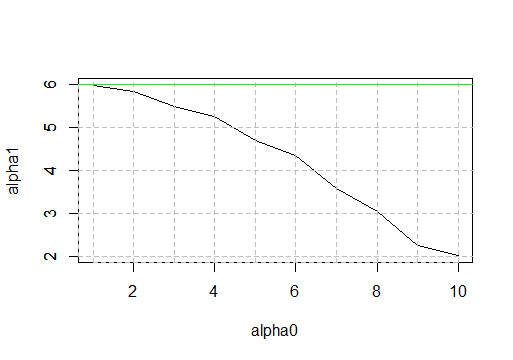
\includegraphics[height=7cm]{graph/alpha1_fct_de_alpha0.png}
 			\caption[Influence de $\alpha_{0}$ dans l'estimation de $\alpha_1$ par inversion du tau de Kendall]{Influence de $\alpha_{0}$ dans l'estimation de $\alpha_1$ par inversion du tau de Kendall : 
 			Cette illustration est générée en simulant $10 \times 10\,000$ observations du modèle collectif du risque présenté dans \cite{Itre5} pour $\alpha_{0} = 1,\dots, 10$, $\alpha_{1}$ demeure constant à $6$ et la copule est logarithmique-logarithmique. La ligne verte correspond au vrai paramètre $\alpha_1$ définit pour les simulations.}
 		\label{graph_alpha1_fct_de_alpha0}
 		\end{figure}
 	
 		Il en résulte que plus la dépendance insérée par la loi mère est forte, moins l'inversion du tau de Kendall constitue un estimateur adéquat de $\alpha_1$.
 		
 		
 		\begin{scenario}\label{scenario_selection_aleatoire_Xij}
 			On sélectionne aléatoirement un $X_{i,j}$ par observation ($i$) afin de calculer $\hat{\beta}$.
 		\end{scenario}
 	
 		Reprenons le scénario \ref{scenario_tous_les_Xij}, mais on définit 
 		$$\hat{\beta} = \frac{(n_{obs}) ^ {n_{sim}}}{\sum_{i=1}^{n_{obs}} \dots \sum_{i=1}^{n_{obs}} x_{i,j}} $$
 		où $j$ est sélectionné aléatoirement entre $\left[1, N_i\right]$ pour chacune des simulations, $n_{sim}$ représente le nombre de simulations et $n_{obs}$ correspond au nombre d'observations dans le jeu de données. Les résultats sont présentés dans le tableau \ref{tbl_resultats_scenario_4}. On voit alors que la méthode \textit{IFM} arrive à des résultats très similaires à ceux de la méthode composite hormis que les temps de calcul sont bien moins longs (11 secondes pour la méthode \textit{IFM} contre 6 minutes pour la composite avec $1\,000$ observations).
 		
 		\begin{table}[H]
 			\centering
 			\begin{tabular}{lcccc}
 				\hline
 				& $q$ & $\beta$ & $\alpha_0$ & $\alpha_1$ \\ 
 				\hline
 				Vrais paramètres & 0.6000 & 0.0100 & 8.0000 & 6.0000 \\ 
 				Méthode \textit{IFM} & 0.6128 & 0.0096 & 8.1509 & 7.1790 \\ 
 				Méthode composite & 0.6130 & 0.0095 & 8.1448 & 7.2790 \\ 
 				Méthode des moments & 0.6128 & 0.0078 & 7.8535 & 4.2966 \\
 				\hline
 			\end{tabular}
 			\caption[Résultats du scénario \ref{scenario_selection_aleatoire_Xij}]{Résultats du scénario \ref{scenario_tous_les_Xij}: La méthode dite \textit{IFM} consiste à trouver les paramètres des distributions marginales, puis à estimer $\hat{\alpha}_{0}$ sachant ces paramètres. De la même façon, on trouve $\hat{\alpha}_{1}$ en fixant $\beta$ et $\alpha_{0}$ comme connus. La méthode dite \textit{composite}, quant à elle, consiste à trouver tous les paramètres simultanément en utilisant la méthode décrite dans la section \ref{sect_seconde_approche}. Finalement, la méthode des moments, dans les cas de $\hat{\alpha}_{0}$ et $\hat{\alpha}_{1}$, consiste à inverser le tau de Kendall empirique.}
 			\label{tbl_resultats_scenario_4}	
 		\end{table}
 	
 	\section{Conclusion}
		 À la suite des scénarios présentés dans ce rapport, on a pu voir que la loi de fréquence avait un impact significatif sur l'estimation des paramètres du modèle collectif du risque. Également, plus la dépendance intégrée par la v.a. mère de la copule archimédienne hiérarchique est forte, plus cela vient biaiser l'estimation du paramètre de la v.a. enfant lorsque l'on utilise la méthode d'inversion du tau de Kendall.
		 Également, on a vu que les fonctions de vraisemblance présentées en \eqref{eq_vrais_alpha1_1} et \eqref{eq_vrais_alpha1_2} ne sont pas adéquates pour estimer le paramètre de dépendance de la loi enfant.\\
		 
		 Dans l'ensemble, peu importe la structure du jeu de données, la méthode composite offre de meilleurs performances que les deux autres approches. Et, surtout, les résultats de cette méthode sont moins influencée par la paramétrisation de $N$ excepté que l'estimation du paramètre de cette dernière variable aléatoire peut être biaisé.\\
		 
		 La prochaine étape de l'étude sera donc de trouver une approche alternative pour estimer le paramètre de dépendance de la v.a. enfant d'une copule archimédienne hiérarchique. Pour récapituler, le temps de dérivation pour obtenir la fonction de vraisemblance complète prend un temps phénoménal à calculer lorsque la v.a. $N$ peut prendre des valeurs supérieures à $5$. Par la suite la méthode d'inversion du tau de Kendall est fortement influencée par le niveau de dépendance induite via la v.a. mère ce qui nous amène à l'exclure aussi. Finalement, la méthode décrite en \eqref{eq_vrais_alpha1_1} et en \eqref{eq_vrais_alpha1_2} ne constitue pas une bonne façon d'estimer le paramètre $\alpha_{1}$ comme il a été illustré dans le présent rapport.
 	

	\newpage
	\bibliography{BibRRT_Kendall.bib}
	\bibliographystyle{apalike}
	
\end{document}